
\section{Feature Evaluation}

Successful classification largely depends on the predictive value of the features. We therefore evaluate for the features whether they will be useful in the discrimination between the formal and informal classes. The evaluation requires the satellite image to be divided into the formal and informal classes. This division is represented using a ground truth, which is a mask covering the satellite image the location of informal areas. The mask is used to divide each block of pixels into the two classes: either formal or informal. Each block contains a vector of features, characterizing that particular block of pixels. All blocks of the same class will be grouped together, allowing for the analysis of the distribution values of the two classes. If the distribution of the values of a certain feature varies substantially between the two classes, it should be a suitable candidate for classification.

The ground truth mask is constructed using a vector file containing the boundaries of informal areas. The boundary file is rasterized and applied on top of the satellite image, creating a mask of the location of the informal areas. Because the feature calculation is performed on blocks instead of pixels, we therefore transform the pixel based mask into a block based mask. In this new block based mask, every pixel represents a block of pixels in the original image. The pixels with the value zero represent formal blocks of pixels while ones represent informal blocks of pixels.

We visualize the predictive value the features using a boxplot and a kernel density estimation plot. When a feature is distinctive, the distribution of the values in the two classes will be different, thus creating a visual difference in both plots. We attempted to use KL divergence as an objective measurement as an alternative for the visual inclined box plot and kernel density estimation. However, we were not able to extract reasonable KL divergence values from our data as for many outcomes would indicate a divergence of infinite value. We will therefore visually evaluate the differences between the formal and informal value distributions in the two types of plots.

The features will be calculated for all combinations of image sections, color bands, block sizes, and scales. This resulted in large amounts of data, of which only a selection will be shown in the following sections. For HoG, LSR and RID the features are extracted from the three sections presented in Figure
\ref{fig:sections} for all three color bands. To analyze the impact of the block size and scale parameters, the block sizes 20, 40 and 60 will be used in combination with the scales 50, 100, 150. The individual
impact of each of the two parameters, is evaluated by the use of a comparison between the baseline and the increased parameter. This is, for example, a comparison between the results obtained from a block size of 20 compared to a block size of 60, with all other parameters constant. This is on the assumption that all parameters are independent from all other parameters.

Because every combination of image section, block size and scale will have three different results due to the RGB color bands, we refrain from visualizing all bands and pick the first band, which is red. The results seem to vary slightly between the red, green, and blue band, although it is not significant. Furthermore, we will select the most expressive feature for each extraction method to reduce the complexity of the visualization.

\subsection{Histogram of Oriented Gradients}

\begin{figure}
\centering
\begin{tabular}{cc}
  \subfloat{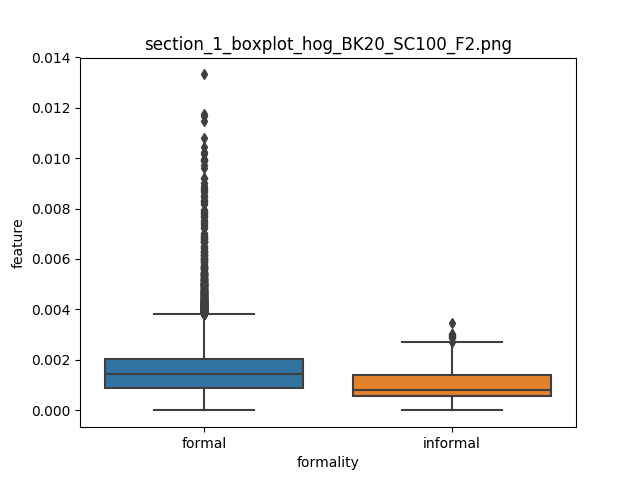
\includegraphics[width=7cm]{images/HoG/inc_bk/section_1_boxplot_hog_BK20_SC100_F2}}&
  \subfloat{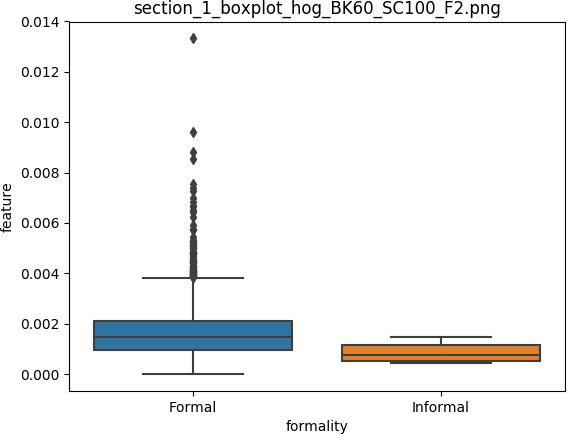
\includegraphics[width=7cm]{images/HoG/inc_bk/section_1_boxplot_hog_BK60_SC100_F2}}\\ 
  \subfloat{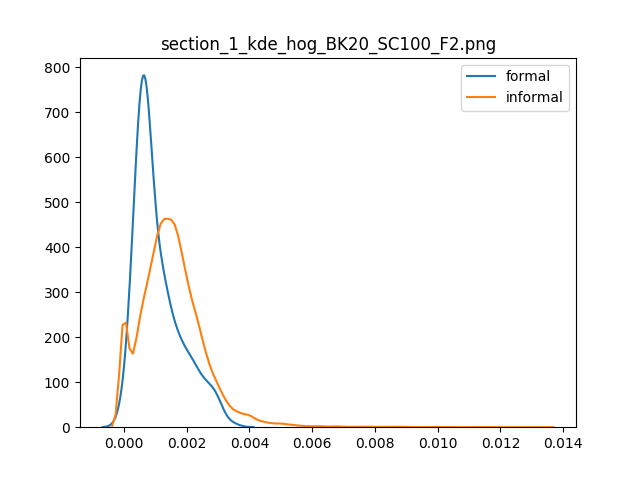
\includegraphics[width=7cm]{images/HoG/inc_bk/section_1_kde_hog_BK20_SC100_F2}}&
  \subfloat{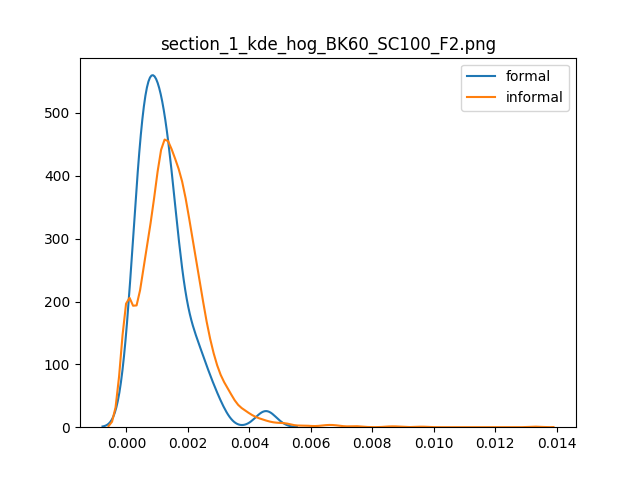
\includegraphics[width=7cm]{images/HoG/inc_bk/section_1_kde_hog_BK60_SC100_F2}}
\end{tabular}
\caption{The effect of increased block size on the HoG features. From left to
right: a block size of 20 and 60 respectively.}
\label{hog_inc_bk}
\end{figure}

For the Histogram of Oriented Gradients, the third feature is selected for visualization in this section. Figure \ref{hog_inc_bk} shows the effect of an increased block size on the distribution of values in both classes. This example uses a constant scale of 100 pixels and a variable block size of 20 and 60 pixels. It seems that the block size, in this case, does not influence the both distributions significantly. As a result an increase in the size of a block within the tested range should have little to no influence on the predictive value of the feature.

\begin{figure}
\centering
\begin{tabular}{cc}
  \subfloat{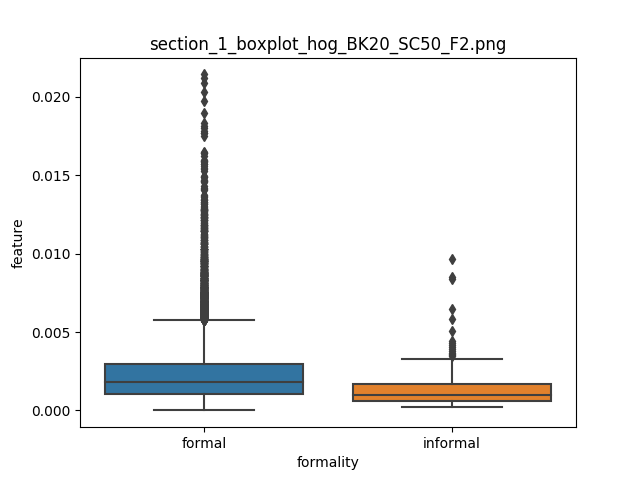
\includegraphics[width=7cm]{images/HoG/inc_sc/section_1_boxplot_hog_BK20_SC50_F2}}&
  \subfloat{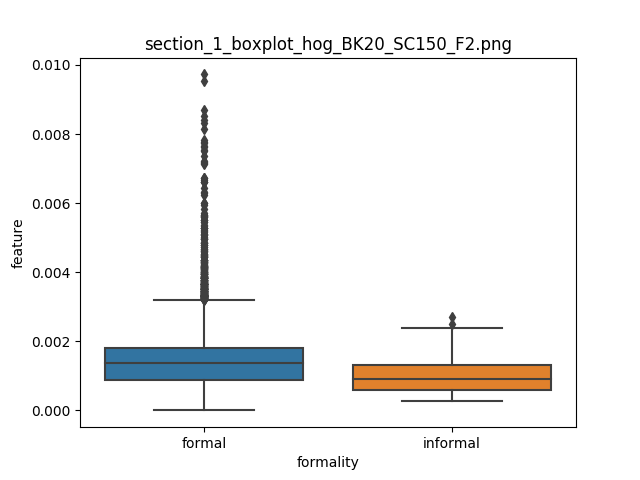
\includegraphics[width=7cm]{images/HoG/inc_sc/section_1_boxplot_hog_BK20_SC150_F2}}\\
  \subfloat{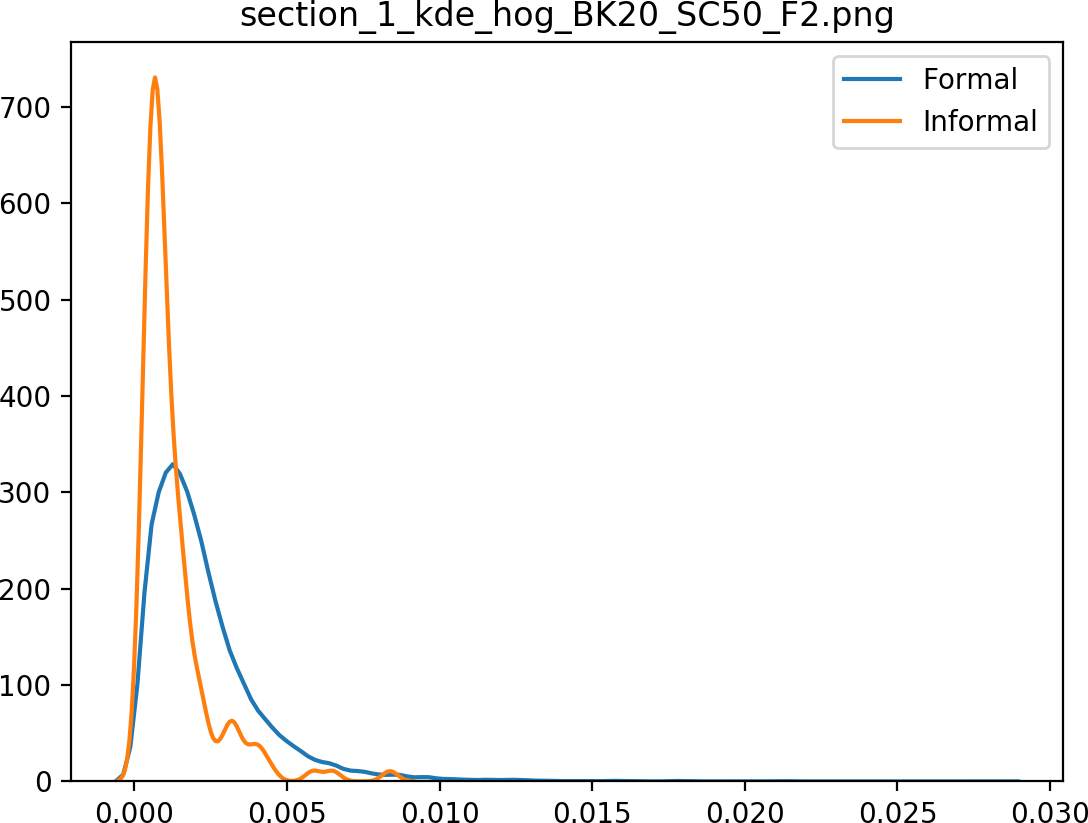
\includegraphics[width=7cm]{images/HoG/inc_sc/section_1_kde_hog_BK20_SC50_F2}}&
  \subfloat{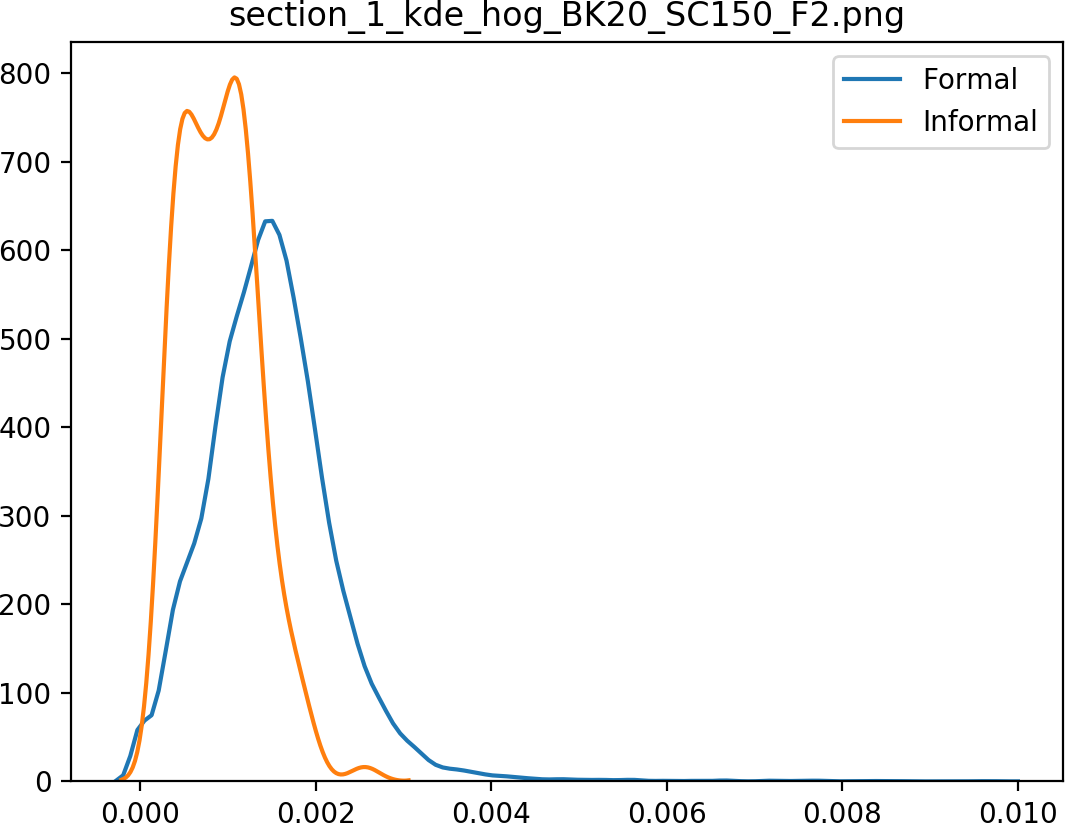
\includegraphics[width=7cm]{images/HoG/inc_sc/section_1_kde_hog_BK20_SC150_F2}}\\
\end{tabular}
\caption{The effect of increased scale on the HoG features. From left to
right: a scale of 50 and 150 respectively}
\label{hog_inc_sc}
\end{figure}

Figure \ref{hog_inc_sc} illustrates the effect of increased scale on a constant block size. It seems to indicate that an increased scale leads to an increased separation of the two distribution, thus increasing the predictive value of the feature. Scales larger than 150 do not seem to improve the performance. In contrast, the performance actually seems to decrease with scales larger than 150. In the paper of Graesser \textit{et al.} combined multiple scales to improve the detection of informal settlements. We will experiment with multiple scales and scale combinations in the results section.

\subsection{Line Support Region}

The Line Support Region feature visualized is the line mean, which was the most expressive of the features. Furthermore, we showed the results from the first section because it produced the most distinct results from the three sections. The individual performances of the different sections will be evaluated in the results section. Similar to the analysis of HoG, the increase of the block size does not seem to influence the distribution of the two classes. The observed difference is as negligible as displayed in the comparison of the HoG in Figure \ref{hog_inc_bk}

\begin{figure}
\centering
\begin{tabular}{cc}
  \subfloat{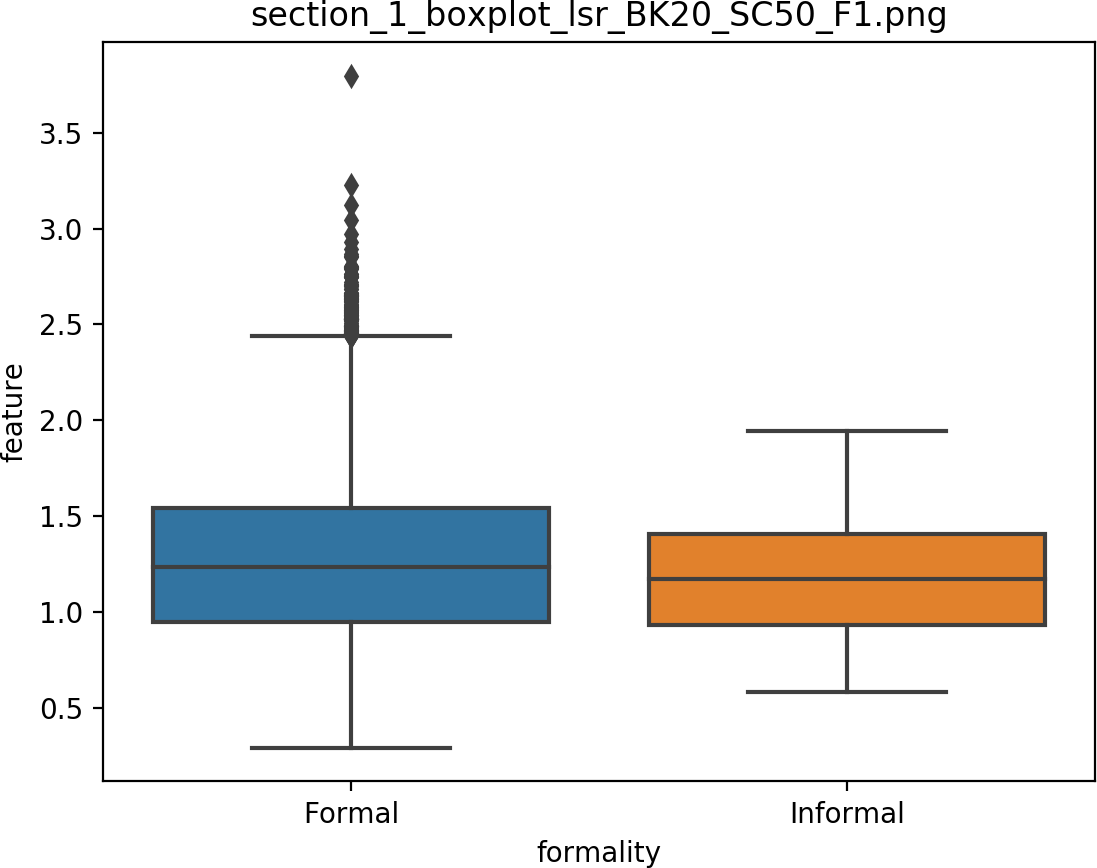
\includegraphics[width=7cm]{images/LSR/inc_sc/section_1_boxplot_lsr_BK20_SC50_F1}}&
  \subfloat{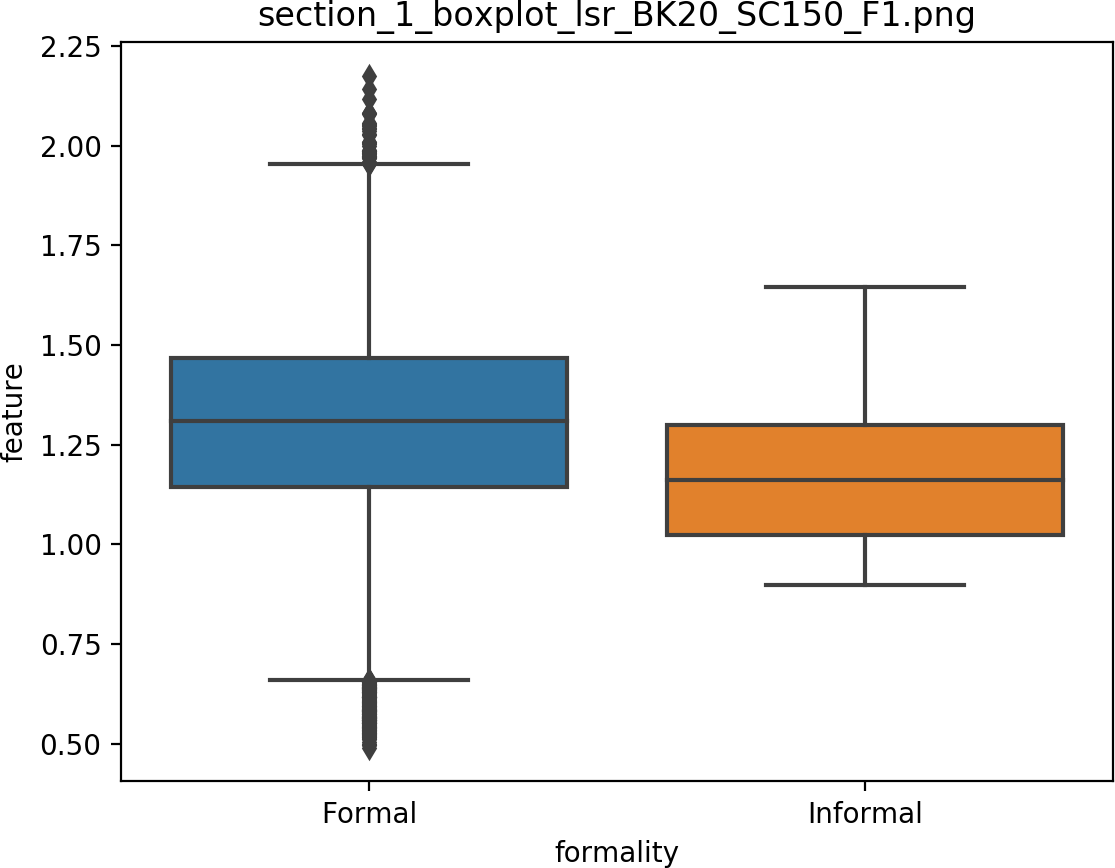
\includegraphics[width=7cm]{images/LSR/inc_sc/section_1_boxplot_lsr_BK20_SC150_F1}}\\
  \subfloat{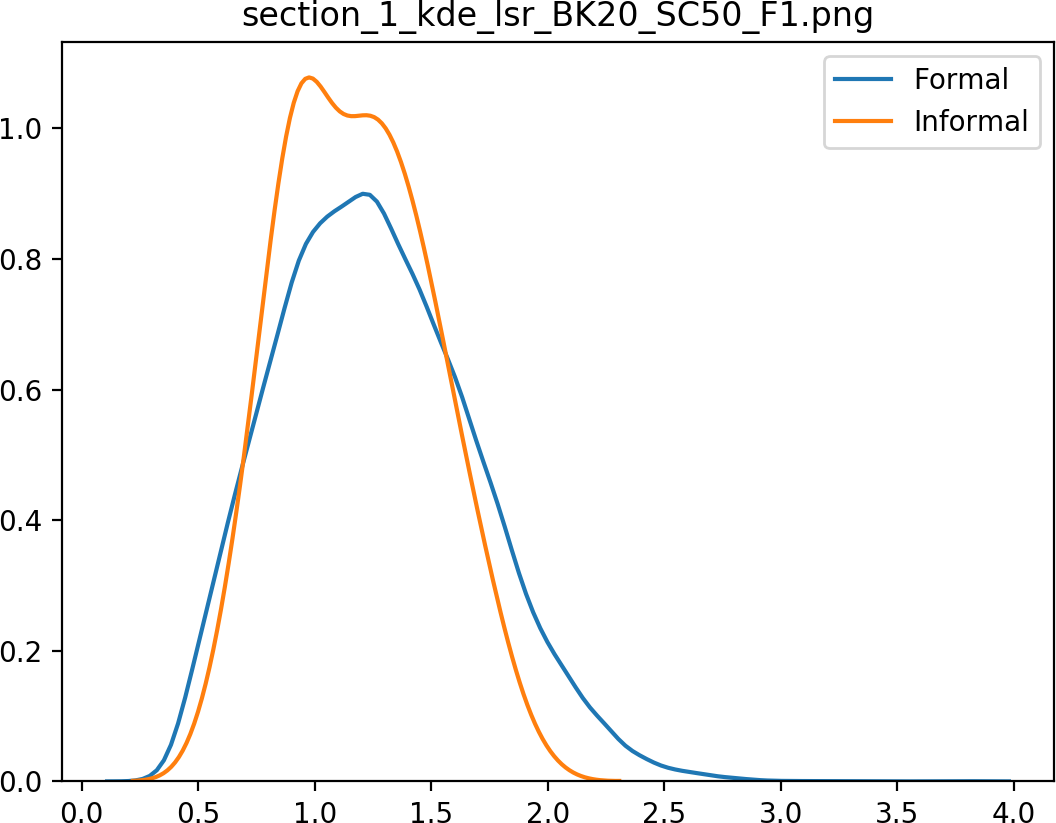
\includegraphics[width=7cm]{images/LSR/inc_sc/section_1_kde_lsr_BK20_SC50_F1}}&
  \subfloat{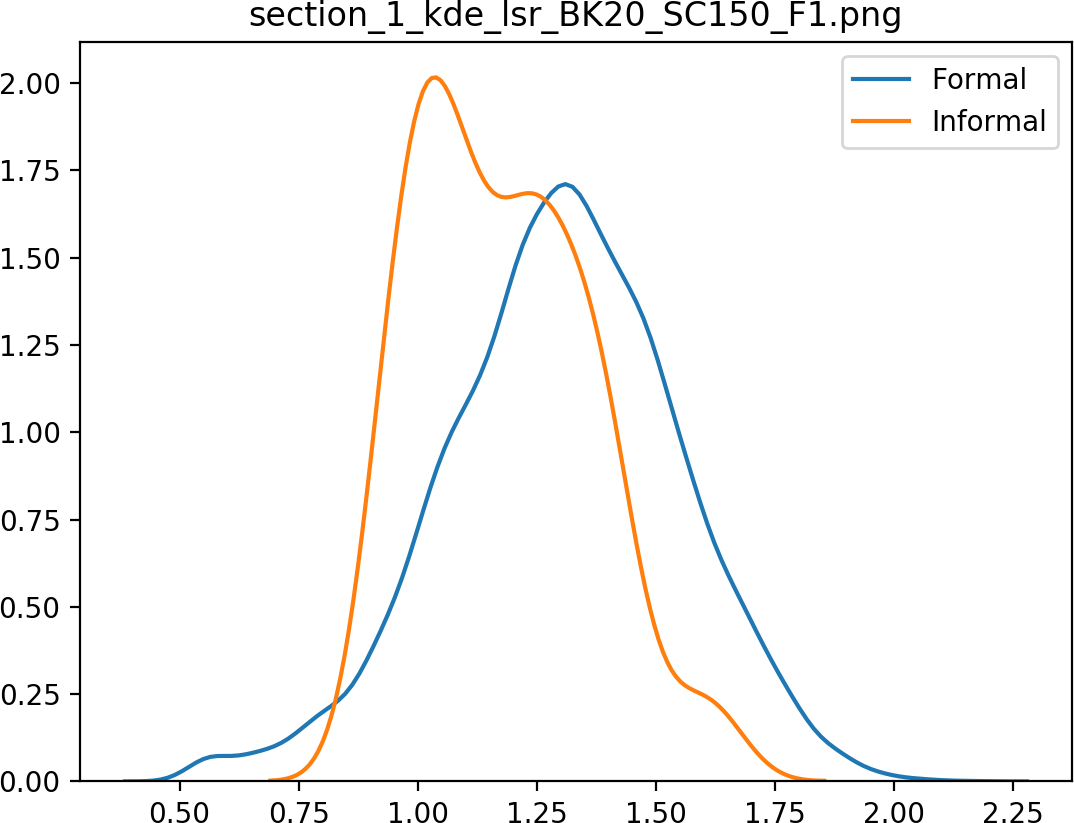
\includegraphics[width=7cm]{images/LSR/inc_sc/section_1_kde_lsr_BK20_SC150_F1}}
\end{tabular}
\caption{The effect of increased scale on the second SLR feature. From left to
right: a scale of 50 and 150 respectively.}
\label{lsr_inc_sc}
\end{figure}

The distributions for different scales of the LSR feature is visualized in Figure \ref{lsr_inc_sc}. Similar to the features from the Histogram of Oriented gradients, it appears that an increase in scale seems to increase the difference between the distributions of the formal and informal classes, although this is not as clear in the other two sections. This seems to indicate that increased scale might improve performance


\subsection{Road Intersection Density}

\begin{figure}
	\centering
	\begin{tabular}{ccc}
		\subfloat{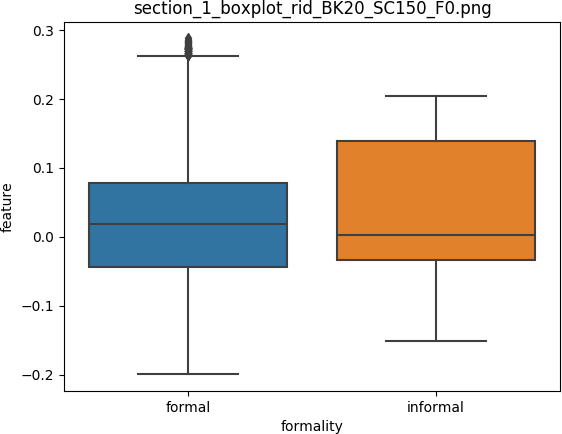
\includegraphics[height=3.8cm]{images/RID/1}}&
		\subfloat{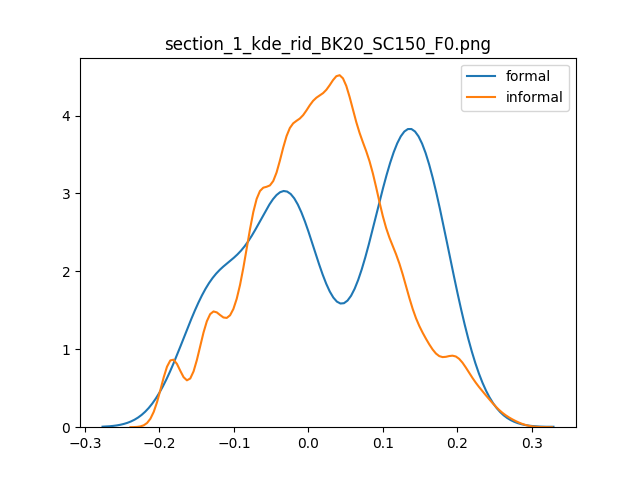
\includegraphics[height=3.8cm]{images/RID/2}}&
		\subfloat{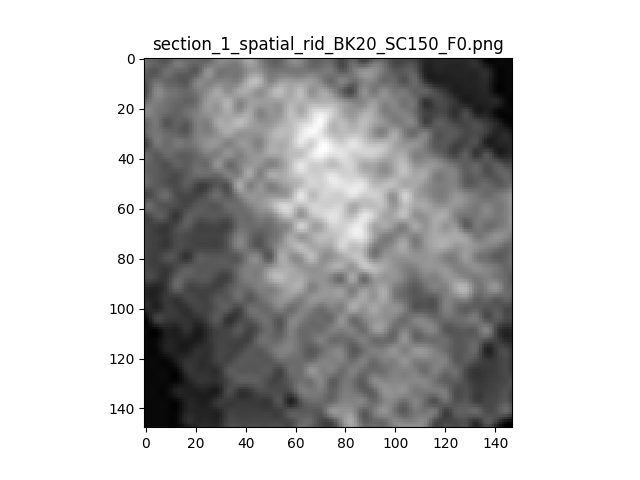
\includegraphics[height=3.8cm]{images/RID/3}}\\
		\subfloat{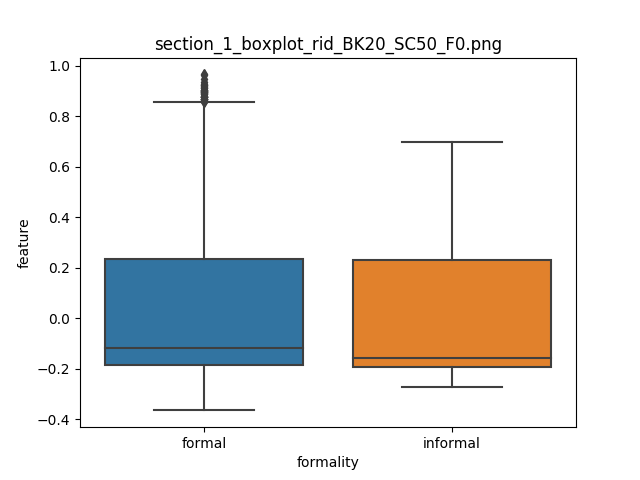
\includegraphics[height=3.8cm]{images/RID/4}}&
		\subfloat{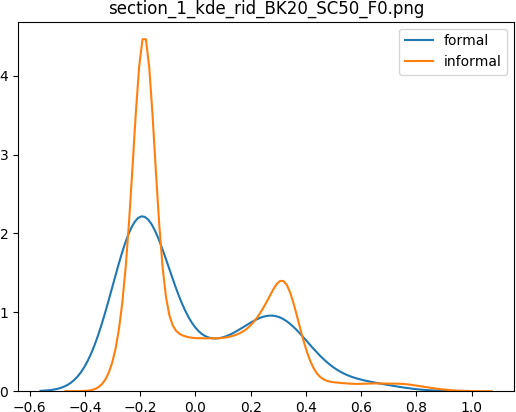
\includegraphics[height=3.8cm]{images/RID/5}}&
		\subfloat{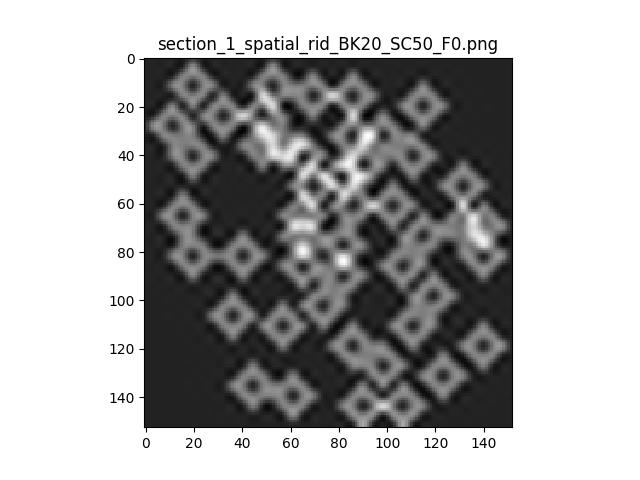
\includegraphics[height=3.8cm]{images/RID/6}}\\
	\end{tabular}
	\caption{The distribution of values for the Road Intersection Density feature. Top: Scale 150; Bottom: Scale 50}
	\label{rid}
\end{figure}


Unlike HoG and LSR, the road intersection density method generates a single feature that is produced by the Gettis and Ord local G function. RID uses different block sizes and scales as well, although, in this case, the meaning of the scale and block size is slightly different. In the calculation of the G function, in order to map the hotspot to the same dimensions of the two other features, the points returned by the intersection detection need to be rasterized onto a grid. This grid has the same dimensions as the two other features, with each block in the grid representing a pixel block in the image. Every block in the grid contains a counter of the number of intersections that fall within that block. The G function is calculated over this grid, resulting in a feature of the correct dimensions. The scale is used in the determination of the neighborhood around a block, just like HoG and LSR although the shape is a circle instead of a square.\newline\newline

\noindent
Figure \ref{rid} shows the differences in distribution for the RID feature for scales 150 and 50. The low scale seems to create artifacts and does not have a distinctly different distribution. The higher scale, on the other hand, does seem to have a difference in distribution, although not quite significant. The other sections have results that are similar to the bottom right image in the figure. In this evaluation, we have only used the parameters that work well with the first section and applied this to the second and third section; this is likely cause for the low performance in the other sections. We would have to use three different sets of parameters to increase performance for the other two sections. It is clear that this approach does not seems scalable to large images where there will be a large variance in the types of roads.

\subsection{Conclusion}

With the right parameters, there is a clear distinction between the two classes for both the HoG and LSR features. RID, in contrast, does not seem to have a clear distinction, likely caused by a lack of specific parameters for section 2 and 3. For HoG and LSR, it seems that an increase in scale improves the distinctness of the two classes, although increased scale is computationally expensive. On the three sections, the time to compute features at a high scale is measured in hours rather than minutes. Using features with high scales on large images would therefore be discouraged. Besides, increasing the scale seems to give diminishing returns while taking significantly more time to compute. We will therefore use 150 as the maximum scale.
For HoG and LSR, the block size did not seem to improve or decrease performance. As a result, we would get the same performance with large block sizes as small block sizes using less computation. For now, the block size remains 20 pixels as the paper by Graesser \textit{et al.} describes. We will test our hypothesis of the effect of block size and scale during the classification experiments in the results section.


